% Created 2017-02-13 Mon 14:23
% Intended LaTeX compiler: pdflatex
\documentclass[presentation]{beamer}
\usepackage[utf8]{inputenc}
\usepackage[T1]{fontenc}
\usepackage{graphicx}
\usepackage{grffile}
\usepackage{longtable}
\usepackage{wrapfig}
\usepackage{rotating}
\usepackage[normalem]{ulem}
\usepackage{amsmath}
\usepackage{textcomp}
\usepackage{amssymb}
\usepackage{capt-of}
\usepackage{hyperref}
\usetheme{CambridgeUS}
\usecolortheme{beaver}
\setcounter{secnumdepth}{1}
\author{Zheng Tian}
\date{}
\title{Lecture 1: What is Econometrics}
\hypersetup{
 pdfauthor={Zheng Tian},
 pdftitle={Lecture 1: What is Econometrics},
 pdfkeywords={},
 pdfsubject={},
 pdfcreator={Emacs 25.1.1 (Org mode 9.0.3)}, 
 pdflang={English}}
\begin{document}

\maketitle
\begin{frame}{Outline}
\setcounter{tocdepth}{1}
\tableofcontents
\end{frame}



\section{What is Econometrics}
\label{sec:orgace6ef0}
\setcounter{tocdepth}{1}
\tableofcontents[currentsection]

\begin{frame}[label={sec:org6ad0bc0}]{What do you think of Econometrics?}
\begin{itemize}
\item Economics?
\item Mathematics?
\item Statistics?
\end{itemize}
\end{frame}


\begin{frame}[label={sec:orgaff73b4}]{Definition of Econometrics}
Stock and Watson (2015) define Econometrics as

\begin{quote}
At a broad level, econometrics is the science and art of using
economic theory and statistical techniques to analyze economic
data.
\end{quote}
\end{frame}


\begin{frame}[label={sec:org1fbec6d}]{Science or art?}
\begin{itemize}
\item The principle of \alert{falsifiability} of scientific research, as Karl Popper
defined.

\begin{figure}[htbp]
\centering
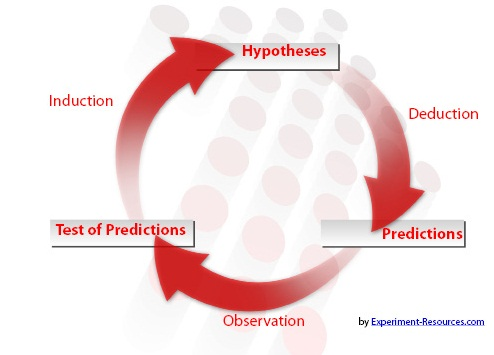
\includegraphics[width=0.6\textwidth,height=0.6\textheight]{figure/reasoning-cycle-research.jpg}
\caption{A reasoning cycle of scientific research}
\end{figure}
\end{itemize}
\end{frame}


\begin{frame}[label={sec:orgb035554}]{Economic theory, statistics, and data}
\begin{itemize}
\item A complete process of econometric research consists of
\begin{itemize}
\item Economic theory
\item Statistical techniques
\item Economic data
\end{itemize}
\end{itemize}

\begin{figure}[htbp]
\centering
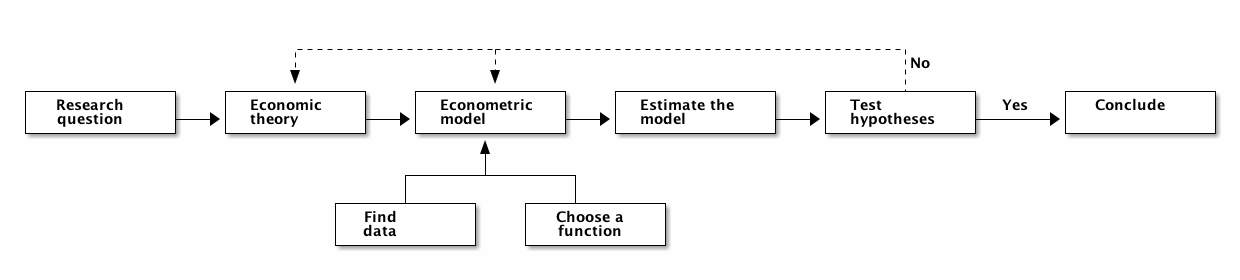
\includegraphics[width=1.0\textwidth]{figure/econometric_workflow.png}
\caption{\label{fig:orga839ddb}
A workflow of econometric research}
\end{figure}
\end{frame}


\section{Economic Questions We Examine}
\label{sec:org059bc82}
\setcounter{tocdepth}{1}
\tableofcontents[currentsection]

\subsection*{Question \#1: Does reducing class size improve elementary school education?}
\label{sec:org9fd08aa}

\begin{frame}[label={sec:org9221c45}]{The argument for small class size goes like this}
Small classes get more teacher-student interaction, fewer disruptions,
and higher grades in test. 

\begin{center}
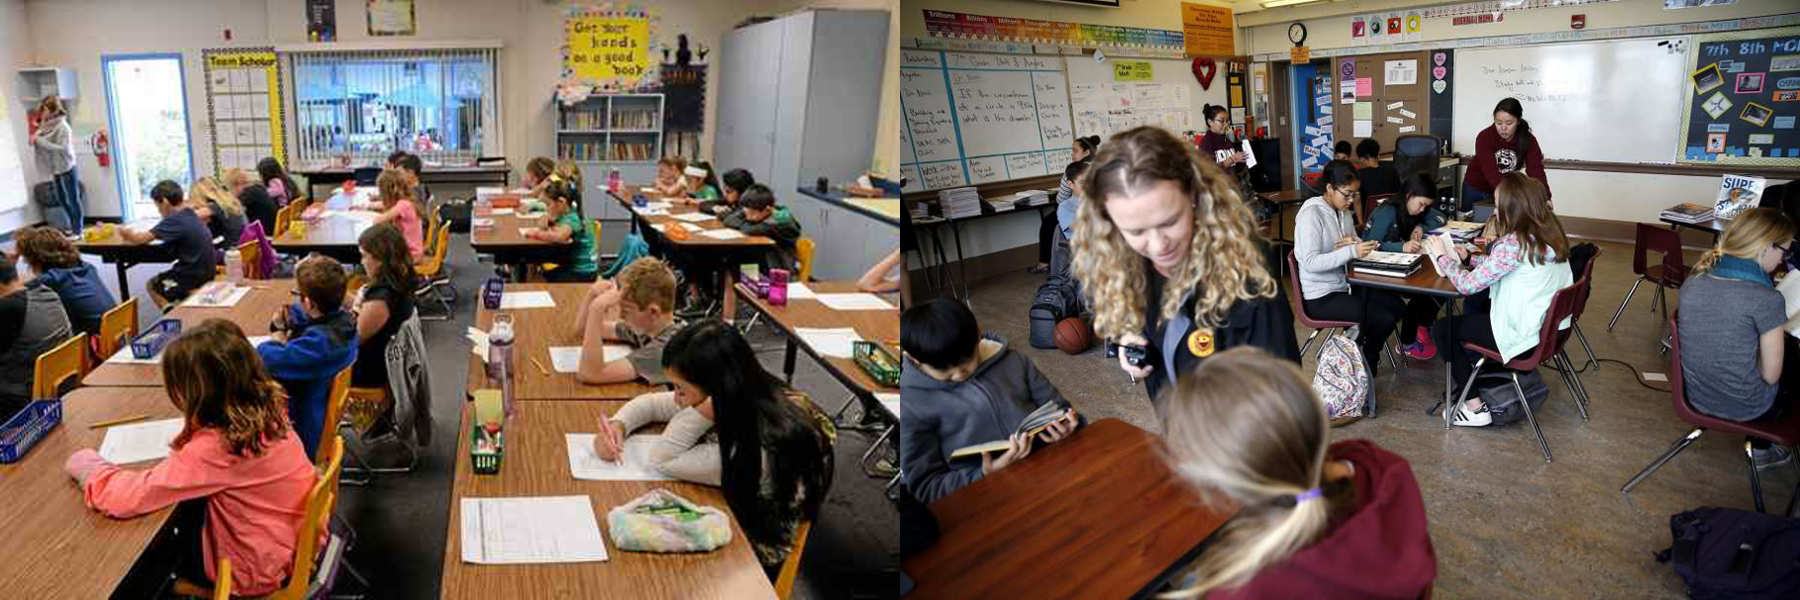
\includegraphics[width=.9\linewidth]{figure/calclassroom_cmp.png}
\end{center}
\end{frame}

\begin{frame}[label={sec:orgca0e4e3}]{The question of interest}
\begin{block}{The research question}
Is there any effect of reducing class size on improving students' grades in
elementary schools?
\end{block}

\begin{block}{Who cares such research?}
\begin{itemize}
\item Teachers
\item Parents
\item School principles
\item Superintendents of school districts
\end{itemize}
\end{block}
\end{frame}

\begin{frame}[label={sec:org10415a5}]{The research design}
\begin{description}
\item[{Qualitative research design}] A field investigation

\item[{Quantitative research design}] Randomized controlled experiments
(RCE, or randomized controlled trial, RCT)
\end{description}
\end{frame}

\begin{frame}[label={sec:org0f3a1c4}]{The sample and data}
\begin{itemize}
\item Draw samples and collect data from 420 California school districts
in 1999.
\item Cross-sectional data. Each row represents a distinct unit of
observation. All observations are collected in a single year.
\end{itemize}

\begin{figure}[htbp]
\centering
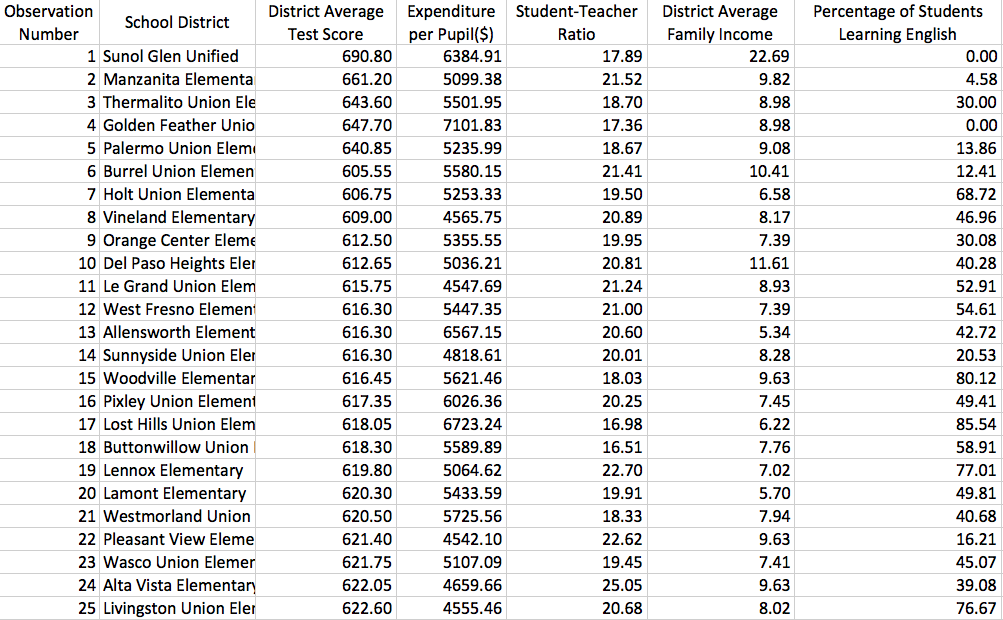
\includegraphics[width=0.6\textwidth,height=0.5\textheight]{figure/table1_1.png}
\caption{\label{fig:orgda30687}
A screen shot of the dataset the California school districts in 1999}
\end{figure}
\end{frame}

\begin{frame}[label={sec:orga9d0a0c}]{The econometric model}
\begin{itemize}
\item Use common sense to build an econometric model in this case.
\item Variables involved: the average test scores in a school district
(\emph{TestScore}) and the student-teacher ratio \emph{STR}.
\item For simplicity, we set up a \alert{simple linear regression
model} as follows,
\end{itemize}

\[ TestScore = \beta_0 + \beta_1 STR + OtherFactors  \]

\begin{itemize}
\item The hypothesis we make is that if \emph{STR} has a non-zero effect on
\emph{TestScore}, that is, \(\beta_1 \neq 0\).

\item The model is then estimated using some estimation method, and we
test the hypothesis with the estimation results using some test
statistics.
\end{itemize}
\end{frame}


\subsection*{Three other questions}
\label{sec:org11c4995}

\begin{frame}[label={sec:orga0eba84}]{The three other questions}
\begin{description}
\item[{Question 1}] Does reducing class size improve elementary school education?
\item[{Question 2}] Is there racial discrimination in the market for home loan?
\item[{Question 3}] How much do cigarette taxes reduce smoking?
\item[{Question 4}] What will the rate of inflation be next year?
\end{description}
\end{frame}

\begin{frame}[label={sec:org31b4265}]{A summary of data types}
\begin{table}[htbp]
\caption{\label{tab:org9040c10}
Data types and econometric methods for all four questions}
\centering
\footnotesize
\begin{tabular}{clp{5cm}}
Questions & Data types & Econometric methods\\
\hline
\#1 & experimental, cross-sectional & multiple regression\\
\#2 & observational, cross-sectional & multiple regression with binary dependent variable\\
\#3 & observational, panel data & Panel data regression model\\
\#4 & observational, time series & multiple regression with lagged dependent variable\\
\end{tabular}
\end{table}
\end{frame}


\section{Causal Effects and Idealized Experiments}
\label{sec:org3176805}
\setcounter{tocdepth}{1}
\tableofcontents[currentsection]

\subsection*{Randomized controlled experiment}
\label{sec:org0cb3305}

\begin{frame}[label={sec:orgb4b8f5f}]{Randomized controlled experiments (or trials, RCTs thereafter)}
\begin{itemize}
\item Clinical trials to test the effectiveness of medical
intervention.
\item All participants are \alert{randomly} assigned into two groups.
\item The control group receives no treatment (or placebo)
\item The treatment group receives the treatment.
\item After a follow-up period, compare the two groups.
\end{itemize}
\end{frame}

\begin{frame}[label={sec:org2afdb73}]{An illustration of RCTs}
\begin{figure}[htbp]
\centering
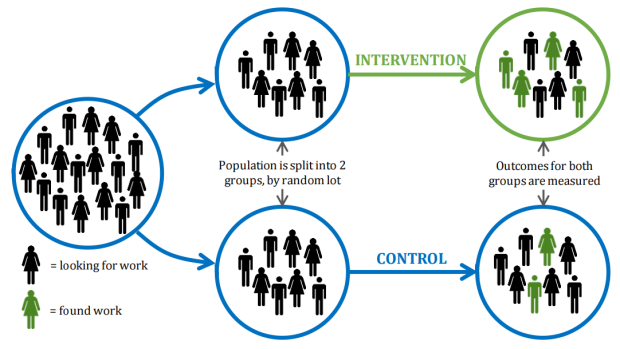
\includegraphics[width=0.8\textwidth,height=0.6\textheight]{figure/rct_example.png}
\caption{\label{fig:orgfb88e5a}
An illustration of a randomized controlled experiment}
\end{figure}
\end{frame}

\begin{frame}[label={sec:org13e74eb}]{The advantage of RCTs}
\begin{itemize}
\item Randomization minimizes selection bias.
\item In the example of California school districts,
randomized control experiments ensure that the only systematic difference
between the classes in the control group and those in the treatment
group is the treatment (reduced class size) itself, with the effects
from other \alert{confounding factors} eliminated.
\end{itemize}
\end{frame}

\begin{frame}[label={sec:orga8685ec}]{The disadvantage of RCTs}
\begin{description}
\item[{Time and costs}] RCTs usually are expensive to undertake and take a
long time to observe the effect of treatment.
\item[{Conflict of interest dangers}] RCTs may be funded by special interest
groups so that its objectivity is doubtful.
\item[{Ethnics}] Especially in social science, we cannot impose some
treatment due to ethnic concerns.
\end{description}
\end{frame}


\begin{frame}[label={sec:org23efa67}]{Causal effect}
\begin{itemize}
\item \alert{Causal effect} is defined to be the effect on an outcome of a given
action or treatment as measured in an ideal RCT.
\item The concept of the ideal randomized controlled experiment does
provide a theoretical benchmark to define causal effects in research
design.
\end{itemize}
\end{frame}


\section{Data Sources and Types}
\label{sec:org9cf4a30}
\setcounter{tocdepth}{1}
\tableofcontents[currentsection]

\begin{frame}[label={sec:org7896b34}]{Experimental versus observational data}
\begin{itemize}
\item \alert{Experimental data} come from experiments designed to evaluate a
treatment or policy or to investigate a causal effect.
\item \alert{Observational (or nonexperimental) data} are collected using
surveys, and administrative records.
\item The problem of using observational data to estimate causal effects is
that the "treatment" is not randomly assigned.
\item Much of econometric methods are developed to deal with
causality using observational data.
\end{itemize}
\end{frame}


\begin{frame}[label={sec:org4a08e8d}]{Cross-sectional data}
\begin{itemize}
\item Data on different entities for a single time period are called
\alert{cross-sectional data}.
\item The sequence of each observation number is arbitrarily assigned.
\item Cross-sectional data can be experimental data or observational data.
\end{itemize}
\end{frame}


\begin{frame}[label={sec:org647b748}]{Time series data}
\begin{itemize}
\item Time series data are data for a single entity collected at multiple
time periods.
\item The sequence of each record is based on the time period
it happened.
\end{itemize}
\end{frame}


\begin{frame}[label={sec:org9928999}]{Panel data}
\begin{itemize}
\item \alert{Panel data}, also called \alert{longitudinal data}, are data for multiple
entities in which \alert{each entity} is observed at two or more time
periods.
\item Panel data are very useful for estimating causal effects.
\end{itemize}
\end{frame}
\end{document}